\section{Разработка информационно-поисковой системы}
\label{sec:development}

\subsection{Выбор средств реализации}

\textbf{Языки программирования, фреймворки и библиотеки}

Информационно-поисковая система (ИПС) реализована по клиент-серверной схеме с
векторной моделью индексирования и поиска. При разработке использован следующий
технологический стек:

\begin{itemize}
	\item \textbf{Python 3.11} "--- основной язык реализации серверной части: бизнес-логика, REST API, обработка текста, оценка качества;
	\item \textbf{Flask 3.0} "--- веб-фреймворк; обеспечивает маршрутизацию HTTP-запросов, раздачу статических файлов фронтенда и реализацию REST API;
	\item \textbf{PostgreSQL 16} "--- реляционная СУБД; хранит документы, логи поиска, словарь и IDF-значения;
	\item \textbf{pgvector} "--- расширение PostgreSQL; хранит TF-IDF-векторы документов и выполняет поиск по косинусной близости;
	\item \textbf{psycopg2-binary} "--- драйвер PostgreSQL для Python;
	\item \textbf{NLTK} "--- библиотека обработки естественного языка; предоставляет стеммер Портера и список стоп-слов английского языка;
	\item \textbf{scikit-learn} "--- используется для подготовки данных и подсчёта метрик качества поиска;
	\item \textbf{matplotlib} "--- построение графиков метрик (точность, полнота, F-мера) для оценки качества;
	\item \textbf{pypdf} "--- извлечение текста из PDF-файлов;
	\item \textbf{python-docx} "--- извлечение текста из DOCX-файлов;
	\item \textbf{watchdog} "--- библиотека мониторинга файловой системы; используется в CLI-клиенте для отслеживания созданий, изменений и удалений файлов в наблюдаемой директории;
	\item \textbf{Docker / Docker Compose} "--- контейнеризация приложения и базы данных, воспроизводимое развёртывание;
	\item \textbf{MinIO Object Storage} "--- S3-совместимое хранилище объектов для оригинальных файлов документов; обеспечивает скачивание файлов через presigned URL или проксирование через Flask с заголовком \texttt{Content-Disposition: attachment};
	\item \textbf{boto3} "--- AWS SDK для Python; используется для взаимодействия с MinIO (загрузка, скачивание, генерация presigned URL);
	\item \textbf{HTML5 / CSS3 / JavaScript (ES6+)} "--- клиентская часть, реализованная статическими файлами без системы сборки.
\end{itemize}

\textbf{Обоснование выбора средств}

Векторная модель поиска (VSM) выбрана в соответствии с заданием как основная модель
описания документов: каждый документ представляется нормированным вектором весов
терминов в пространстве словаря размерности $D$, а релевантность запросу оценивается
косинусной близостью векторов. Это позволяет ранжировать результаты по убыванию
релевантности и оценивать качество поиска стандартными метриками.

Flask выбран как лёгкий и гибкий веб-фреймворк: система не требует асинхронной
обработки больших потоков запросов, а статический фронтенд и REST API обслуживаются
одним процессом без дополнительной инфраструктуры. PostgreSQL с расширением pgvector
избавляет от необходимости хранить векторы и выполнять скалярные вычисления близости
в приложении: оператор \texttt{<=>} (косинусное расстояние) выполняется на стороне
СУБД, что упрощает реализацию и повышает производительность поиска.

Использование NLTK обусловлено готовыми компонентами предобработки: стеммер Портера
приводит словоформы к основе, а встроенный список стоп-слов исключает неинформативные
термины ("the", "is", "at" и т.~п.). Библиотеки pypdf и python-docx позволяют расширить
поддерживаемые форматы загружаемых документов без реализации собственных парсеров.
Контейнеризация Docker обеспечивает воспроизводимость окружения и простоту
развёртывания в локальной вычислительной сети: сервис приложения публикуется на порту
5000 и доступен всем узлам сети. Библиотека watchdog используется в отдельном
CLI-клиенте для мониторинга файловой системы и автоматической репликации изменений
на сервер.

\subsection{Описание используемых готовых компонентов}

Особенности применения готовых компонентов в разработанной системе:

\begin{itemize}
	\item \textbf{pgvector} "--- расширение добавляет тип данных \texttt{vector(5000)} и оператор \texttt{<=>} для косинусного расстояния. Вектор каждого документа хранится непосредственно в таблице \texttt{documents}; поиск выполняется одним SQL-запросом с сортировкой по близости и ограничением \texttt{LIMIT}. Недостаток "--- фиксированная размерность вектора задаётся при создании таблицы и должна совпадать с размерностью словаря в коде приложения;
	\item \textbf{NLTK} "--- используются \texttt{stopwords.words('english')} и \texttt{PorterStemmer}. Данные стоп-слов и токенизации загружаются при сборке Docker-образа, что исключает сетевые запросы во время работы;
	\item \textbf{Flask} "--- используется в режиме разработки (встроенный сервер); статические страницы отдаются через \texttt{send\_from\_directory}. Для боевого развёртывания рекомендуется WSGI-сервер (gunicorn);
	\item \textbf{matplotlib} "--- агрегируется в фоновом режиме (\texttt{Agg}); график метрик формируется на сервере и передаётся клиенту в виде base64-изображения, что не требует хранения файлов;
	\item \textbf{scikit-learn} "--- применяется для подсчёта метрик классификации (точность, полнота, F-меры) при оценке качества поиска;
	\item \textbf{pypdf / python-docx} "--- подключаются динамически внутри стратегии загрузчика документов; при отсутствии библиотеки пользователю возвращается понятное сообщение об ошибке;
	\item \textbf{Docker Compose} "--- оркестрация трёх сервисов (\texttt{db}, \texttt{app}, \texttt{minio}) с проверкой готовности базы данных (healthcheck) и автоматическим применением миграций при старте. MinIO предоставляет объектное хранилище для оригинальных файлов документов (bucket \texttt{documents}).
\end{itemize}

\subsection{Структура разработанной системы}

Система состоит из трёх уровней: клиентского (веб-интерфейс), серверного (Flask-приложение)
и уровня данных (PostgreSQL). Основной сценарий работы системы "--- обработка поискового
запроса "--- представлен диаграммой последовательности на рисунке~\ref{fig:architecture}.

\begin{figure}[H]
	\centering
	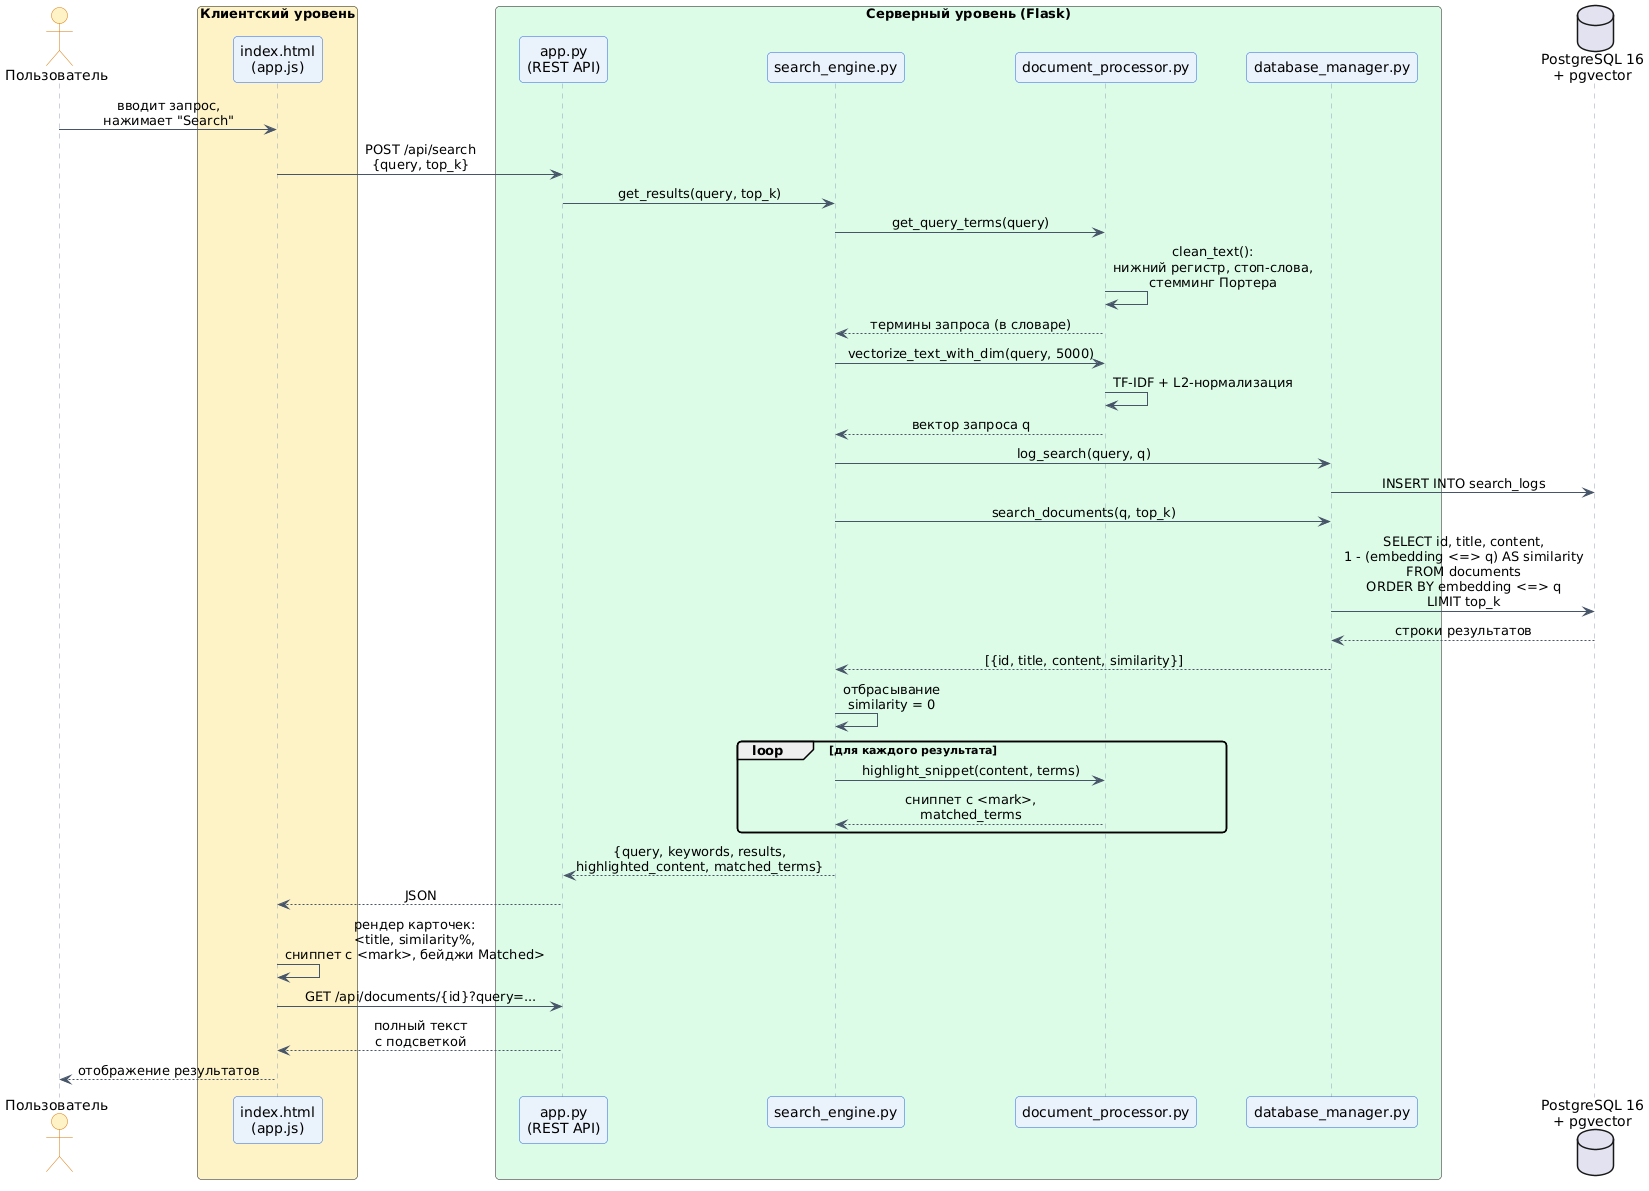
\includegraphics[width=1.0\textwidth]{png/sequence_search.png}
	\caption{Диаграмма последовательности обработки поискового запроса.}
	\label{fig:architecture}
\end{figure}

Серверная часть разбита на модули по принципу разделения ответственности:

\begin{itemize}
	\item \texttt{app.py} "--- точка входа; регистрирует REST-эндпоинты (\texttt{/api/search}, \texttt{/api/upload}, \texttt{/api/upload-file}, \texttt{/api/documents}, \texttt{/api/documents/<id>/download}, \texttt{/api/metrics}, \texttt{/api/stats}, \texttt{/api/help}, \texttt{/api/init-db}) и раздаёт статические страницы; при старте инициализирует bucket MinIO;
	\item \texttt{search\_engine.py} "--- оркестрация поиска: векторизация запроса, вызов векторного поиска в БД, формирование сниппетов с подсветкой релевантных терминов;
	\item \texttt{document\_processor.py} "--- предобработка текста, построение словаря, вычисление IDF, TF-IDF-векторизация, подсветка терминов;
	\item \texttt{document\_loader.py} "--- стратегия загрузки файлов: извлечение текста из различных форматов (\texttt{.txt}, \texttt{.md}, \texttt{.pdf}, \texttt{.docx}, \texttt{.html}, \texttt{.rtf}, \texttt{.csv}, \texttt{.log});
	\item \texttt{database\_manager.py} "--- все операции с PostgreSQL: CRUD документов (включая колонку \texttt{s3\_key} для хранения ключа в MinIO), векторный поиск, логирование запросов, сохранение/загрузка словаря и IDF;
	\item \texttt{s3\_client.py} "--- S3-клиент для MinIO: загрузка файлов (\texttt{upload\_file}), скачивание (\texttt{download\_file}), генерация presigned URL, проверка существования объектов, управление bucket;
	\item \texttt{evaluator.py} "--- вычисление метрик качества (точность, полнота, F-меры) и построение графиков;
	\item \texttt{watch\_handler.py} "--- серверная обработка событий файлового наблюдателя: извлечение текста, сохранение оригинального файла в MinIO, пересчёт словаря/IDF, генерация саммари, векторизация и upsert/delete документа;
	\item \texttt{migrate.py} "--- собственный раннер SQL-миграций, отслеживающий применённые миграции в таблице \texttt{schema\_migrations}.
\end{itemize}

Клиентский уровень реализован пятью статическими страницами: поиск (\texttt{index.html}),
загрузка документов (\texttt{upload.html}), просмотр документов (\texttt{documents.html}),
оценка качества (\texttt{metrics.html}) и справка (\texttt{help.html}). Взаимодействие
с сервером осуществляется через \texttt{fetch} по REST API с JSON-телом.

\subsection{Файловый наблюдатель (File Watcher)}

Для автоматической репликации изменений файловой системы на сервер реализован
отдельный CLI-клиент (\texttt{file\_watcher/watch\_client.py}), работающий на базе
библиотеки \texttt{watchdog}. Клиент выполняется на стороне пользователя (вне Docker-контейнера)
и взаимодействует с сервером через HTTP POST-запросы к эндпоинту \texttt{/api/watch-event}.

Архитектура клиента включает три основных компонента:

\begin{itemize}
	\item \textbf{WatchEventHandler} "--- обработчик событий watchdog (\texttt{on\_created}, \texttt{on\_modified}, \texttt{on\_deleted}, \texttt{on\_moved}); фильтрует файлы по расширению, выполняет debounce-задержку и отправляет HTTP POST на сервер;
	\item \textbf{WatchState} "--- персистентное состояние в файле \texttt{.watch\_state.json} (путь \texttt{<dir>/.watch\_state.json}); хранит \texttt{\{filepath: \{mtime, size\}\}} для каждого индексированного файла; при запуске клиент сравнивает текущее состояние файловой системы с сохранённым и отправляет только разницу (новые, изменённые, удалённые файлы);
	\item \textbf{CLI (argparse)} "--- интерфейс командной строки с параметрами: директория, адрес сервера, client-id, рекурсивный режим, расширения файлов, debounce, путь к state-файлу.
\end{itemize}

Потоки данных клиента:

\begin{enumerate}
	\item \textbf{При запуске:} загрузка \texttt{.watch\_state.json}, сканирование директории (\texttt{os.walk}), сравнение с сохранённым состоянием, отправка diff'а (new/changed/deleted) серверу, обновление state-файла;
	\item \textbf{При работе:} watchdog Observer отслеживает события в реальном времени; при каждом событии (\texttt{on\_created}/\texttt{on\_modified}/\texttt{on\_deleted}) клиент отправляет POST-запрос на сервер и обновляет \texttt{.watch\_state.json}.
\end{enumerate}

На сервере обработка событий выполняется модулем \texttt{watch\_handler.py}, который
вызывается из REST API (\texttt{/api/watch-event}). Для событий \texttt{created} и
\texttt{modified}: извлекается текст (через \texttt{document\_loader.py}), пересчитываются
словарь и IDF по всему корпусу, генерируется саммари, вычисляется TF-IDF-вектор и
выполняется upsert документа в БД. Для события \texttt{deleted}: документ удаляется
по \texttt{file\_path}, после чего пересчитываются словарь и IDF.

Последовательность взаимодействия компонентов при работе файлового наблюдателя
приведена на рисунке~\ref{fig:watch_seq}.

\begin{figure}[H]
	\centering
	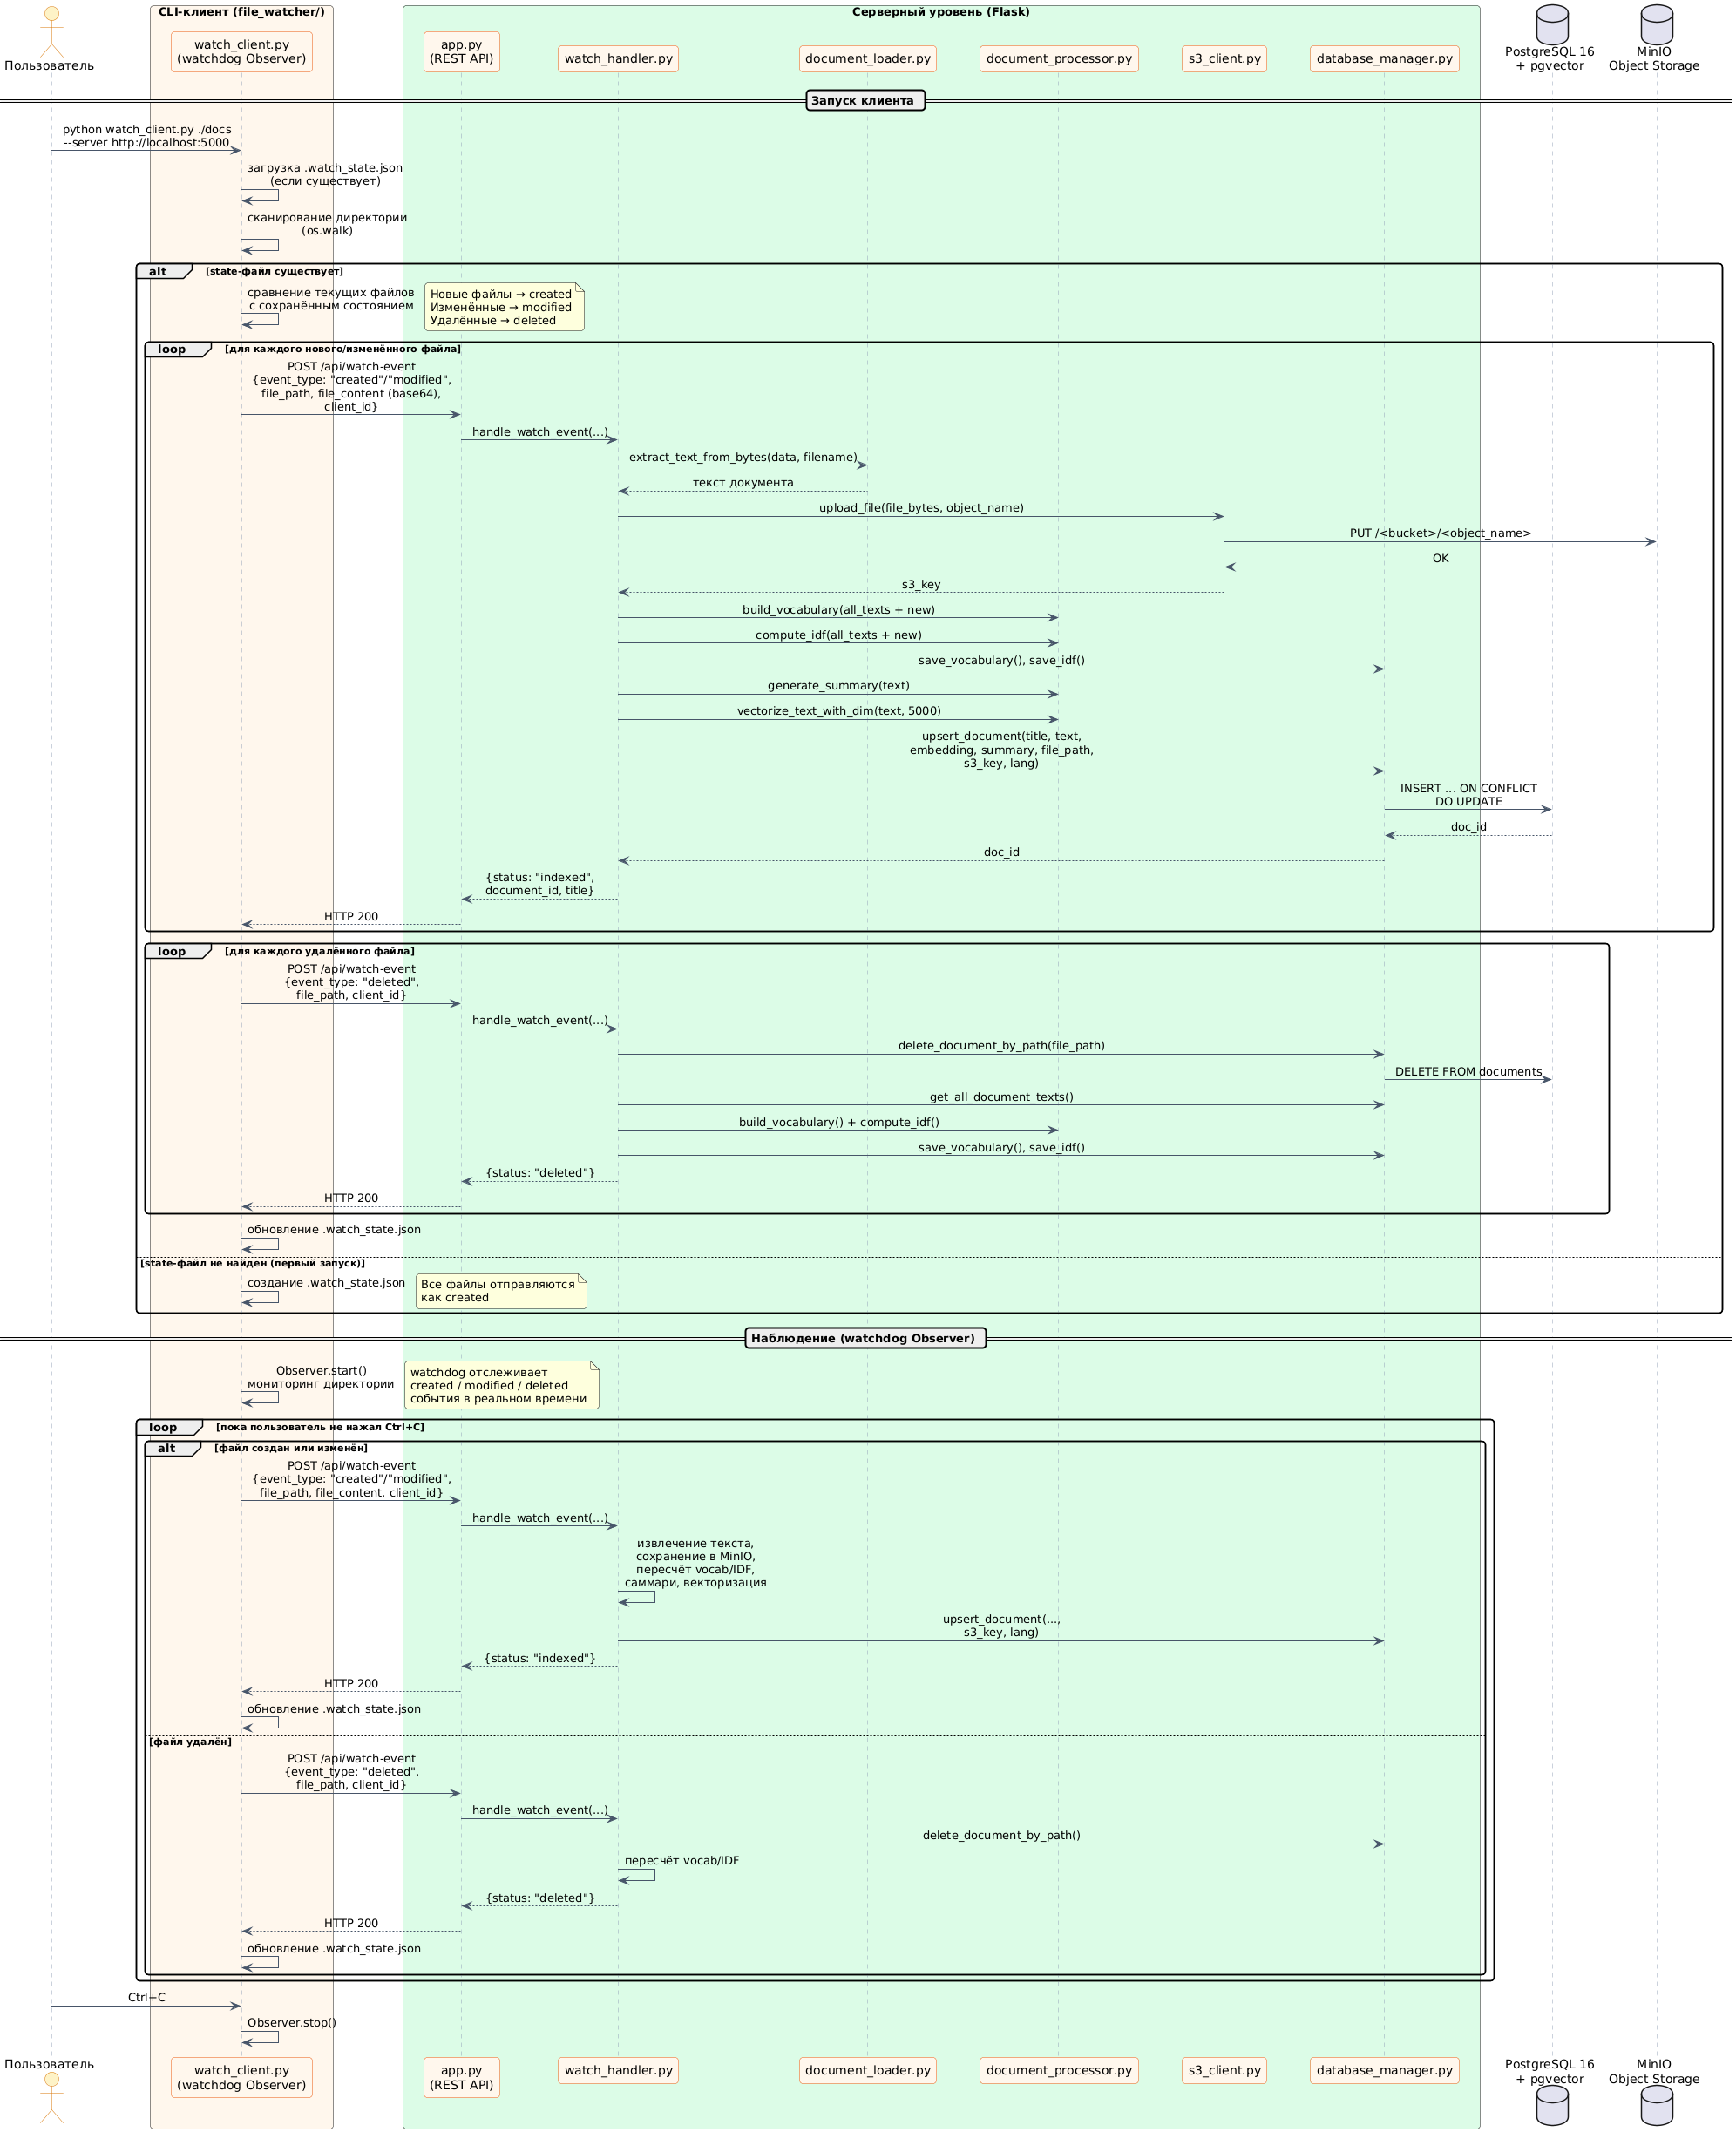
\includegraphics[width=1.0\textwidth]{png/sequence_watch.png}
	\caption{Диаграмма последовательности работы файлового наблюдателя.}
	\label{fig:watch_seq}
\end{figure}

\subsection{Хранение и скачивание документов (MinIO S3)}

Для хранения оригинальных файлов документов используется MinIO Object Storage "--- 
S3-совместимое хранилище объектов. При загрузке файла через \texttt{/api/upload-file}
или при обработке событий файлового наблюдателя оригинальный файл сохраняется в MinIO
(bucket \texttt{documents}), а в таблицу \texttt{documents} записывается ключ объекта
(\texttt{s3\_key}) в формате \texttt{<uuid>.<ext>}.

Скачивание документов реализовано через эндпоинт \texttt{/api/documents/<id>/download}.
При наличии \texttt{s3\_key} файл скачивается из MinIO через \texttt{s3\_client.py}
и отдаётся пользователю с заголовком \texttt{Content-Disposition: attachment}, что
обеспечивает скачивание файла вместо отображения в браузере. Для старых документов
без \texttt{s3\_key} (загруженных через текстовый ввод) генерируется \texttt{.txt}-файл
на лету из сохранённого текста.

Архитектура взаимодействия при скачивании документа представлена на рисунке~\ref{fig:download_seq}.

\begin{figure}[H]
	\centering
	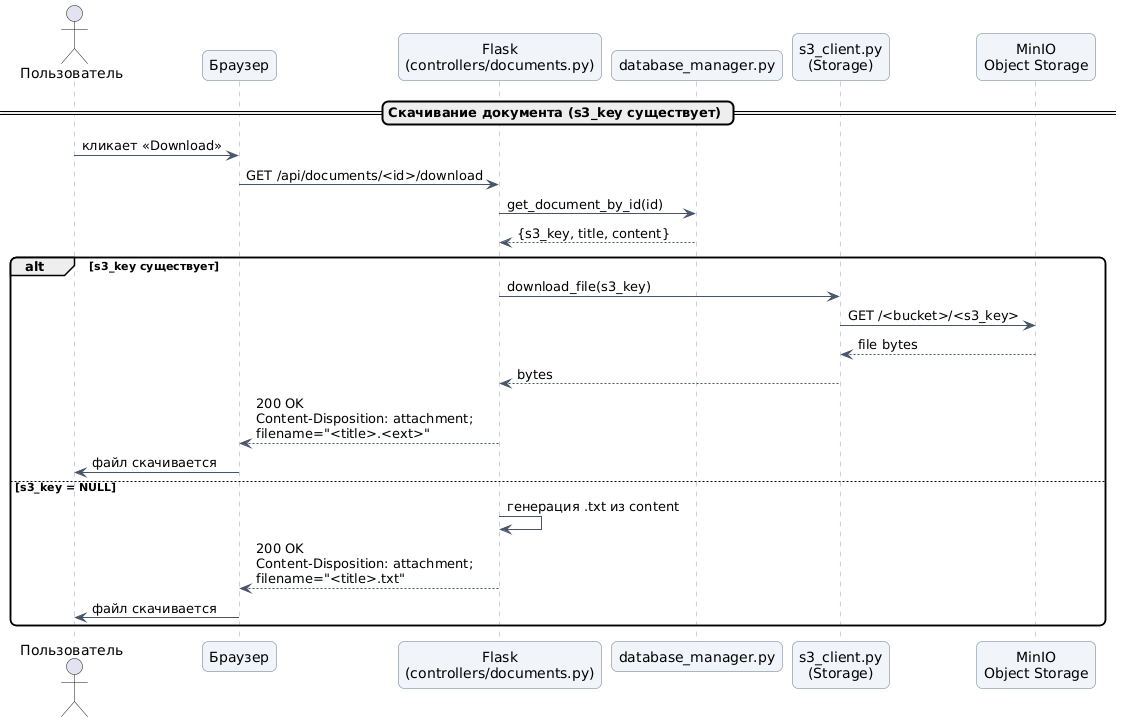
\includegraphics[width=1.0\textwidth]{png/sequence_download.png}
	\caption{Диаграмма последовательности скачивания документа из MinIO.}
	\label{fig:download_seq}
\end{figure}

Последовательность загрузки файла в MinIO при загрузке через веб-интерфейс
представлена на рисунке~\ref{fig:upload_file_seq}.

\begin{figure}[H]
	\centering
	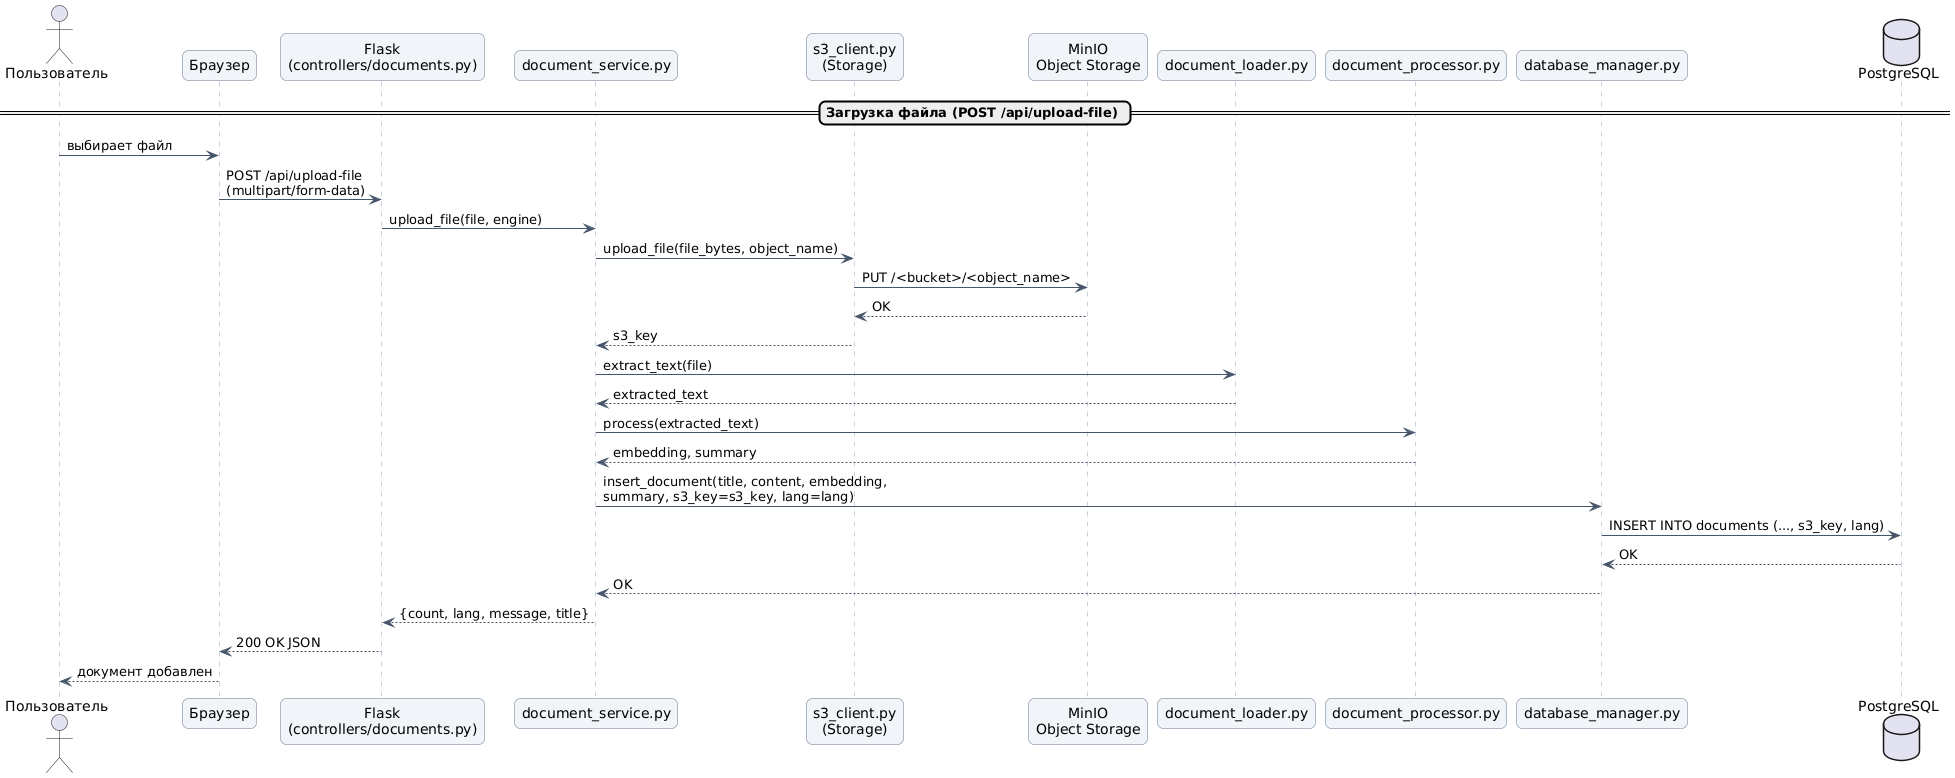
\includegraphics[width=1.0\textwidth]{png/sequence_upload_file.png}
	\caption{Диаграмма последовательности загрузки файла с сохранением в MinIO.}
	\label{fig:upload_file_seq}
\end{figure}

Развёртывание выполняется в Docker Compose: сервис \texttt{db} (образ \texttt{pgvector/pgvector:pg16}),
сервис \texttt{app} (образ на основе \texttt{python:3.11-slim}) и сервис \texttt{minio}
(образ \texttt{quay.io/minio/minio}). При старте контейнера \texttt{app} ожидается
готовность базы данных, применяются миграции, создаётся bucket \texttt{documents} в MinIO,
запускается Flask, а затем автоматически инициализируется корпус документов (если база пуста).
Приложение доступно по \texttt{http://<host>:5000}, MinIO Console "--- по \texttt{http://<host>:9001},
что позволяет использовать систему в локальной вычислительной сети.

\subsection{Структура базы данных системы}

База данных содержит семь таблиц, перечисленных в таблице~\ref{tab:db_tables}.

\begin{table}[H]
	\centering
	\begin{tabular}{|p{3.2cm}|p{8.8cm}|}
		\hline
		\textbf{Таблица} & \textbf{Назначение} \\
		\hline
		\texttt{documents} & Индексированные документы: идентификатор, заголовок, полный текст, дата добавления, TF-IDF-вектор размерности 5000, саммари, путь к файлу, код языка (\texttt{lang}: \texttt{en}/\texttt{fr}), ключ объекта в MinIO (\texttt{s3\_key}) \\
		\hline
		\texttt{search\_logs} & Логи поисковых запросов: текст запроса, вектор запроса, время \\
		\hline
		\texttt{vocabulary} & Словарь терминов: слово и его индекс в векторе \\
		\hline
		\texttt{idf\_values} & Инверсные документные частоты терминов словаря \\
		\hline
		\texttt{schema\_migrations} & Служебная таблица учёта применённых миграций \\
		\hline
		\texttt{watch\_clients} & Зарегистрированные клиенты-наблюдатели: ID, наблюдаемая директория, время регистрации \\
		\hline
		\texttt{watch\_events} & Логи событий файлового наблюдателя: тип события, путь к файлу, время \\
		\hline
	\end{tabular}
	\caption{Таблицы базы данных и их назначение.}
	\label{tab:db_tables}
\end{table}

Словарь и IDF-значения хранятся в базе данных для персистентности между перезапусками
приложения, однако при выполнении поиска используются их in-memory копии (глобальные
структуры \texttt{VOCAB} и \texttt{IDF}), что исключает обращения к БД при каждом
векторном поиске.

\subsection{Основные алгоритмы реализации компонентов}

\textbf{Предобработка текста.} Исходный текст приводится к нижнему регистру, из него
удаляются цифры, пунктуация и спецсимволы; для французского режима сохраняются
диакритические символы (\texttt{àâäéèêëîïôöùûüç"{o}e}). Затем токены
фильтруются по списку стоп-слов (соответствующий набор для каждого языка
из NLTK) и стеммируются алгоритмом Портера (только для английского;
французский текст не стемминуется, чтобы сохранить окончания). Параметр
\texttt{lang} устанавливается автоматически при загрузке документа
(классификатор записывает результат в колонку \texttt{lang} таблицы
\texttt{documents}) и при поиске определяется для запроса тем же
классификатором. Результат "--- список основ терминов, из которых
строятся векторы.

\textbf{Построение словаря и вычисление IDF.} Словарь формируется как упорядоченное
множество уникальных терминов корпуса; мощность словаря определяет размерность
векторного пространства $D$. Инверсная документная частота вычисляется по формуле:

\begin{equation}
	B_{i} = \log\left(\frac{N}{P_{i} + 1}\right) + 1,
	\label{eq:idf}
\end{equation}

где $N$ "--- число документов в коллекции; $P_{i}$ "--- число документов, содержащих
термин $i$. Добавление единицы в знаменатель и к результату устраняет нулевые значения
для терминов, встречающихся во всех документах, сохраняя свойство убывания значимости
частых терминов.

\textbf{TF-IDF-векторизация.} Вес термина $i$ в документе $j$ вычисляется по формуле:

\begin{equation}
	A^{j}_{i} = Q^{j}_{i} \times B_{i},
	\label{eq:weight}
\end{equation}

где $Q^{j}_{i} = 1 + \log\left(\text{tf}^{j}_{i}\right)$ "--- сглаженная частота термина
в документе (логарифмическая нормализация снижает влияние часто повторяющихся слов).
Полученный вектор нормируется евклидовой нормой:

\begin{equation}
	\vec{v} = \frac{\vec{w}}{\lVert \vec{w} \rVert}.
	\label{eq:norm}
\end{equation}

Ключевой фрагмент векторизации приведён в листинге~\ref{lst:vectorize}.

\begin{lstlisting}[caption={Функция TF-IDF-векторизации текста.},label={lst:vectorize}]
def vectorize_text_with_dim(text: str, dim: int, lang: str = 'en') -> List[float]:
    tokens = clean_text(text, lang)
    tf = Counter(tokens)
    vector = [0.0] * dim
    for token, count in tf.items():
        if token in VOCAB:
            idx = VOCAB[token]
            if idx < dim:
                tf_val = 1 + math.log(count) if count > 0 else 0
                idf_val = IDF.get(token, math.log(10) + 1)
                vector[idx] = tf_val * idf_val
    norm = math.sqrt(sum(v * v for v in vector))
    if norm > 0:
        vector = [v / norm for v in vector]
    return vector
\end{lstlisting}

\textbf{Модель поиска.} Запрос пользователя обрабатывается той же функцией
векторизации, что и документы, после чего релевантность документа $d$ запросу $q$
оценивается косинусной близостью соответствующих векторов:

\begin{equation}
	\operatorname{sim}(d, q) = \frac{(\vec{D}, \vec{Q})}{\lVert \vec{D} \rVert \cdot \lVert \vec{Q} \rVert}.
	\label{eq:cosine}
\end{equation}

Поскольку документные векторы нормированы, косинусная близость равна скалярному
произведению. В СУБД это реализовано оператором pgvector \texttt{<=>} (косинусное
расстояние), а итоговая оценка близости вычисляется как разность единицы и косинусного
расстояния (листинг~\ref{lst:search}): $\operatorname{sim}(d,q) = 1 - d_{\cos}(\vec{D}, \vec{Q})$.

\begin{lstlisting}[caption={Векторный поиск в PostgreSQL (pgvector).},label={lst:search}]
SELECT id, title, content,
       1 - (embedding <=> %s::vector) AS similarity
FROM documents
ORDER BY embedding <=> %s::vector
LIMIT %s
\end{lstlisting}

Результаты с нулевой близостью отбрасываются: они не несут информации для
пользователя и засоряют выдачу.

\textbf{Подсветка релевантных терминов.} Для каждого результата строится сниппет:
находится первое вхождение термина запроса (после стемминга), вокруг него выделяется
окно фиксированной длины с многоточиями по краям, а все совпавшие термины оборачиваются
в HTML-тег \texttt{<mark>}. Если ни один термин запроса не встречается в документе,
подсвечиваются ключевые термины самого документа (по весу TF-IDF). Подсветка также
применяется при просмотре полного текста документа по клику.

\textbf{Загрузка документов.} Модуль \texttt{document\_loader.py} реализует стратегию
извлечения текста по расширению файла: текстовые форматы декодируются с перебором
кодировок (UTF-8, CP1251, Latin-1), HTML очищается от тегов и скриптов, RTF "--- от
управляющих слов, PDF и DOCX обрабатываются библиотеками pypdf и python-docx.
Поддерживаемые форматы перечислены в таблице~\ref{tab:formats}.

\begin{table}[H]
	\centering
	\begin{tabular}{|p{4.5cm}|p{7.5cm}|}
		\hline
		\textbf{Расширение} & \textbf{Механизм извлечения текста} \\
		\hline
		\texttt{.txt}, \texttt{.md}, \texttt{.csv}, \texttt{.log} & декодирование с перебором кодировок \\
		\hline
		\texttt{.pdf} & библиотека pypdf (постраничное извлечение) \\
		\hline
		\texttt{.docx} & библиотека python-docx (абзацы и таблицы) \\
		\hline
		\texttt{.html}, \texttt{.htm} & удаление тегов и script/style-блоков \\
		\hline
		\texttt{.rtf} & удаление управляющих слов RTF \\
		\hline
	\end{tabular}
	\caption{Поддерживаемые форматы загружаемых документов.}
	\label{tab:formats}
\end{table}

При загрузке каждого нового документа определяется его язык трёхметодным
классификатором (результат записывается в колонку \texttt{lang} таблицы
\texttt{documents}); далее словарь и IDF пересчитываются по всему корпусу
и сохраняются в базу данных, после чего документ индексируется (его TF-IDF-вектор
вставляется в таблицу \texttt{documents}). Последовательность взаимодействия компонентов
при индексировании документа приведена на рисунке~\ref{fig:indexing}.

\begin{figure}[H]
	\centering
	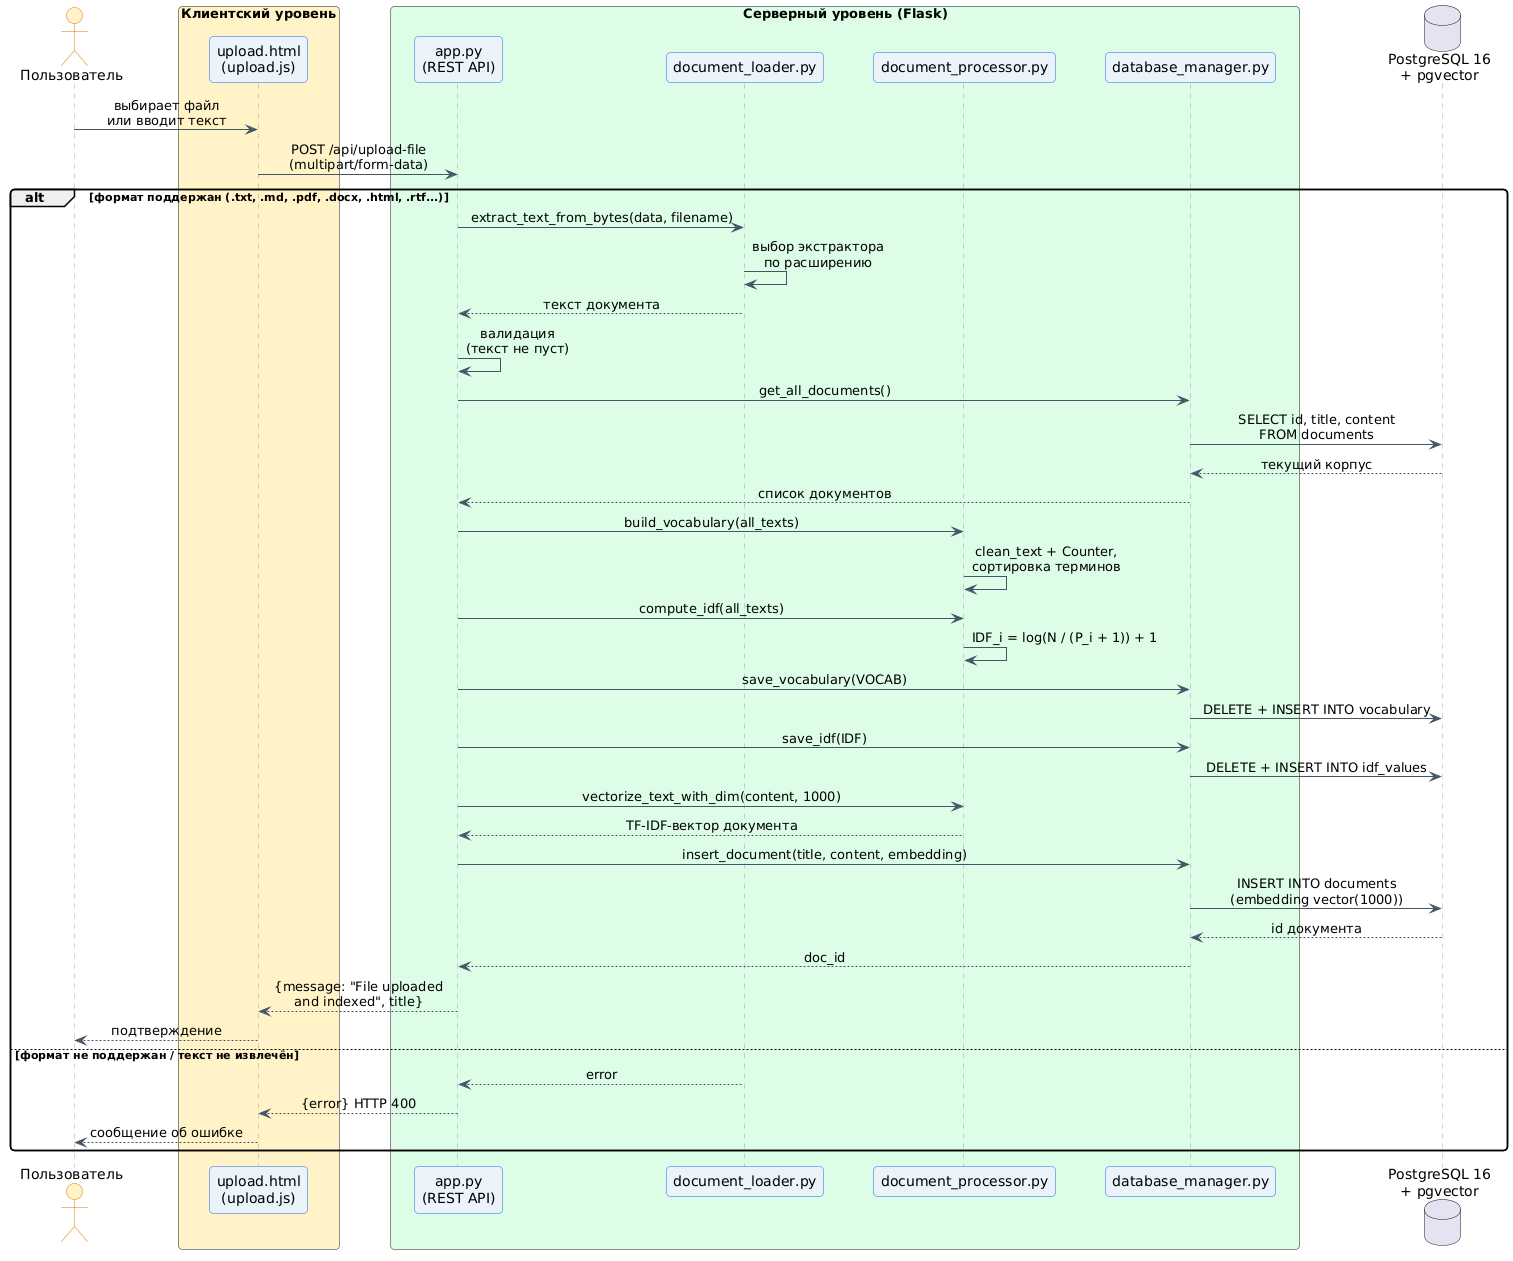
\includegraphics[width=1.0\textwidth]{png/sequense_indexing.png}
	\caption{Диаграмма последовательности индексирования документа.}
	\label{fig:indexing}
\end{figure}

\textbf{Оценка качества поиска.} Для оценки качества используются метрики точности,
полноты и F-меры, вычисляемые по множествам выданных и релевантных документов:

\begin{equation}
	P = \frac{|R \cap Rel|}{|R|}, \qquad
	R = \frac{|R \cap Rel|}{|Rel|},
	\label{eq:pr}
\end{equation}

\begin{equation}
	F_{\beta} = \frac{(1 + \beta^{2}) \cdot P \cdot R}{\beta^{2} \cdot P + R}.
	\label{eq:fbeta}
\end{equation}

Параметр $\beta$ позволяет сместить акцент: $\beta = 0{,}5$ "--- важнее точность,
$\beta = 1$ "--- сбалансированная F1-мера, $\beta = 2$ "--- важнее полнота.
Оценка выполняется автоматически: для каждого тестового запроса выполняется реальный
поиск (извлекаются \texttt{retrieved\_ids}), которые сравниваются с эталонными
релевантными документами, заданными пользователем на странице \texttt{metrics.html}.
Последовательность взаимодействия компонентов при оценке качества приведена
на рисунке~\ref{fig:metrics_seq}.

\begin{figure}[H]
	\centering
	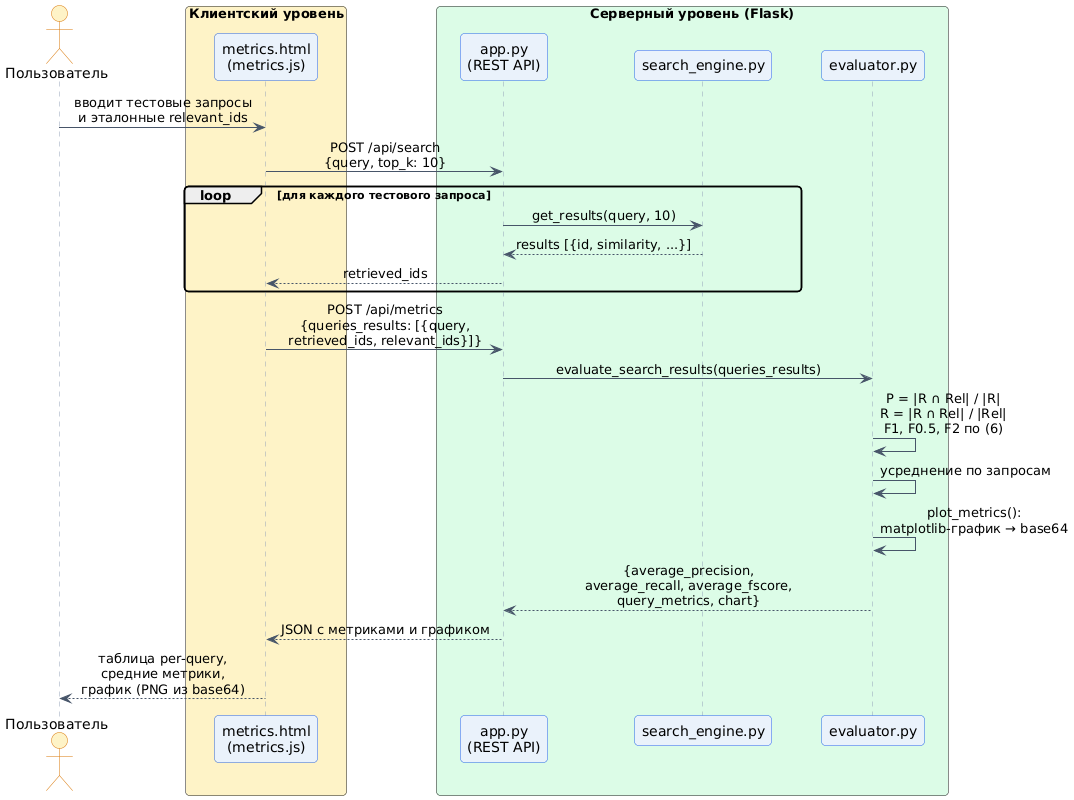
\includegraphics[width=1.0\textwidth]{png/sequence_metrics.png}
	\caption{Диаграмма последовательности оценки качества поиска.}
	\label{fig:metrics_seq}
\end{figure}

\subsection{Информация о тестовой коллекции документов}

Тестовая коллекция состоит из 12 текстовых документов на английском языке объёмом
по 300 "--- 600 слов каждый, посвящённых тематике музыки. Перечень документов приведён
в таблице~\ref{tab:collection}.

\begin{table}[H]
	\centering
	\begin{tabular}{|c|p{4.8cm}|p{6.8cm}|}
		\hline
		\textbf{ID} & \textbf{Документ} & \textbf{Тематика} \\
		\hline
		1 & blues\_music & блюз: происхождение, исполнители, влияние \\
		\hline
		2 & classical\_music & классическая музыка: эпохи, композиторы \\
		\hline
		3 & electronic\_music & электронная музыка: синтезаторы, жанры \\
		\hline
		4 & jazz\_music & джаз: история, инструменты, музыканты \\
		\hline
		5 & music\_concerts & концерты: организация, живое исполнение \\
		\hline
		6 & music\_education & музыкальное образование и обучение \\
		\hline
		7 & music\_industry & музыкальная индустрия и бизнес \\
		\hline
		8 & music\_instruments & музыкальные инструменты и их классификация \\
		\hline
		9 & music\_production & музыкальное производство и запись \\
		\hline
		10 & music\_theory & теория музыки: ритм, мелодия, гармония \\
		\hline
		11 & pop\_music & популярная музыка и её особенности \\
		\hline
		12 & rock\_music & рок-музыка: жанры, инструменты, история \\
		\hline
	\end{tabular}
	\caption{Тестовая коллекция документов.}
	\label{tab:collection}
\end{table}

Документы загружаются в систему автоматически при первой инициализации базы данных
(\texttt{/api/init-db}) и хранятся в каталоге \texttt{backend/documents/} в формате
\texttt{.txt}.

\subsection{Результаты тестирования системы}

Тестирование проводилось вручную по следующим сценариям:

\begin{enumerate}
	\item инициализация базы данных: миграции применяются в правильном порядке, корпус из 12 документов загружается автоматически при пустой базе и не дублируется при повторных стартах;
	\item поиск по запросам различной длины: одиночный термин, многокомпонентный запрос, запрос с отсутствующими в корпусе словами; проверялись релевантность выдачи, корректность процента близости и отбрасывание нулевых результатов;
	\item подсветка релевантных терминов: в сниппетах и в полном тексте документа помечаются термины запроса; для документов без совпадений применяется фолбэк по ключевым терминам документа;
	\item загрузка документов: ручной ввод текста, загрузка \texttt{.txt}, \texttt{.pdf}, \texttt{.docx}, \texttt{.html}; проверялось извлечение текста и индексация; неподдерживаемый формат (например, \texttt{.png}) отклоняется с понятным сообщением;
	\item просмотр и удаление документов: список с идентификаторами, открытие полного текста, удаление;
	\item скачивание документов: для документов с \texttt{s3\_key} файл скачивается из MinIO с заголовком \texttt{Content-Disposition: attachment}; для документов без \texttt{s3\_key} генерируется \texttt{.txt}-файл на лету;
	\item оценка качества: для набора тестовых запросов рассчитываются точность, полнота и F-меры, строится график;
	\item файловый наблюдатель: запуск клиента с наблюдаемой директорией; проверяется автоматическая индексация новых файлов, обновление изменённых, удаление удалённых; проверяется корректность state-файла при перезапуске;
	\item отказоустойчивость: недоступность базы данных, пустой запрос, пустой файл, файл без извлекаемого текста.
\end{enumerate}

В ходе тестирования были выявлены и устранены следующие дефекты:

\begin{itemize}
	\item страница оценки метрик отправляла на сервер поле \texttt{relevantIds} вместо ожидаемого \texttt{relevant\_ids} и не передавала \texttt{retrieved\_ids}, из-за чего сервер завершался с ошибкой \texttt{KeyError}; исправлено: фронтенд выполняет реальный поиск и передаёт оба списка, на сервере добавлен фолбэк "--- при отсутствии \texttt{retrieved\_ids} поиск выполняется автоматически;
	\item сниппеты результатов обрезались до 500 символов на уровне SQL-запроса, что не позволяло строить осмысленную подсветку; полный текст теперь возвращается целиком, а обрезка выполняется при формировании сниппета;
	\item при повторном старте контейнера корпус документов дублировался; добавлена проверка числа документов перед инициализацией.
\end{itemize}

Все сценарии после исправлений проходят успешно.

\subsection{Результаты оценки по метрикам}

Оценка выполнялась на тестовой коллекции из 12 документов. Для каждого из 11 тестовых
запросов задавалось эталонное множество релевантных документов (1 "--- 3 документа).
Система выполняла реальный поиск (топ-10), после чего вычислялись метрики. Результаты
приведены в таблице~\ref{tab:metrics}.

\begin{table}[H]
	\centering
	\begin{tabular}{|p{5.2cm}|c|c|c|c|c|}
		\hline
		\textbf{Запрос} & \textbf{P} & \textbf{R} & \textbf{F1} & \textbf{F0.5} & \textbf{F2} \\
		\hline
		jazz saxophone trumpet & 1,000 & 1,000 & 1,000 & 1,000 & 1,000 \\
		\hline
		blues & 0,667 & 1,000 & 0,800 & 0,714 & 0,909 \\
		\hline
		rock electric guitar & 0,500 & 1,000 & 0,667 & 0,556 & 0,833 \\
		\hline
		concerts live & 0,250 & 1,000 & 0,400 & 0,294 & 0,625 \\
		\hline
		classical music symphony & 0,200 & 1,000 & 0,333 & 0,238 & 0,556 \\
		\hline
		electronic music & 0,200 & 1,000 & 0,333 & 0,238 & 0,556 \\
		\hline
		pop music & 0,100 & 1,000 & 0,182 & 0,122 & 0,357 \\
		\hline
		music production recording & 0,100 & 1,000 & 0,182 & 0,122 & 0,357 \\
		\hline
		music theory harmony & 0,100 & 1,000 & 0,182 & 0,122 & 0,357 \\
		\hline
		music education & 0,100 & 1,000 & 0,182 & 0,122 & 0,357 \\
		\hline
		music industry & 0,100 & 1,000 & 0,182 & 0,122 & 0,357 \\
		\hline
		\textbf{Среднее} & \textbf{0,302} & \textbf{1,000} & \textbf{0,404} & \textbf{0,321} & \textbf{0,533} \\
		\hline
	\end{tabular}
	\caption{Метрики качества поиска по тестовым запросам.}
	\label{tab:metrics}
\end{table}

Аналитическая интерпретация. Полнота $R = 1{,}0$ для всех запросов: при небольшом
корпусе (12 документов) и выдаче из 10 результатов все эталонные релевантные документы
всегда попадают в топ-10, т.~е. система не теряет ни одного релевантного документа.
Точность $P$ убывает от 1,0 (запрос с редкими терминами \texttt{jazz saxophone trumpet})
до 0,1 (общие запросы \texttt{pop music}, \texttt{music theory harmony}), поскольку
документы корпуса тематически близки и делят значительную часть словаря "--- по общим
запросам в топ-10 попадает много нерелевантных документов с ненулевой близостью.
Средняя F1-мера составила 0,404: при идеальной полноте качество ограничивает именно
точность.

Графическое представление результатов приведено на рисунке~\ref{fig:metrics}.

\begin{figure}[H]
	\centering
	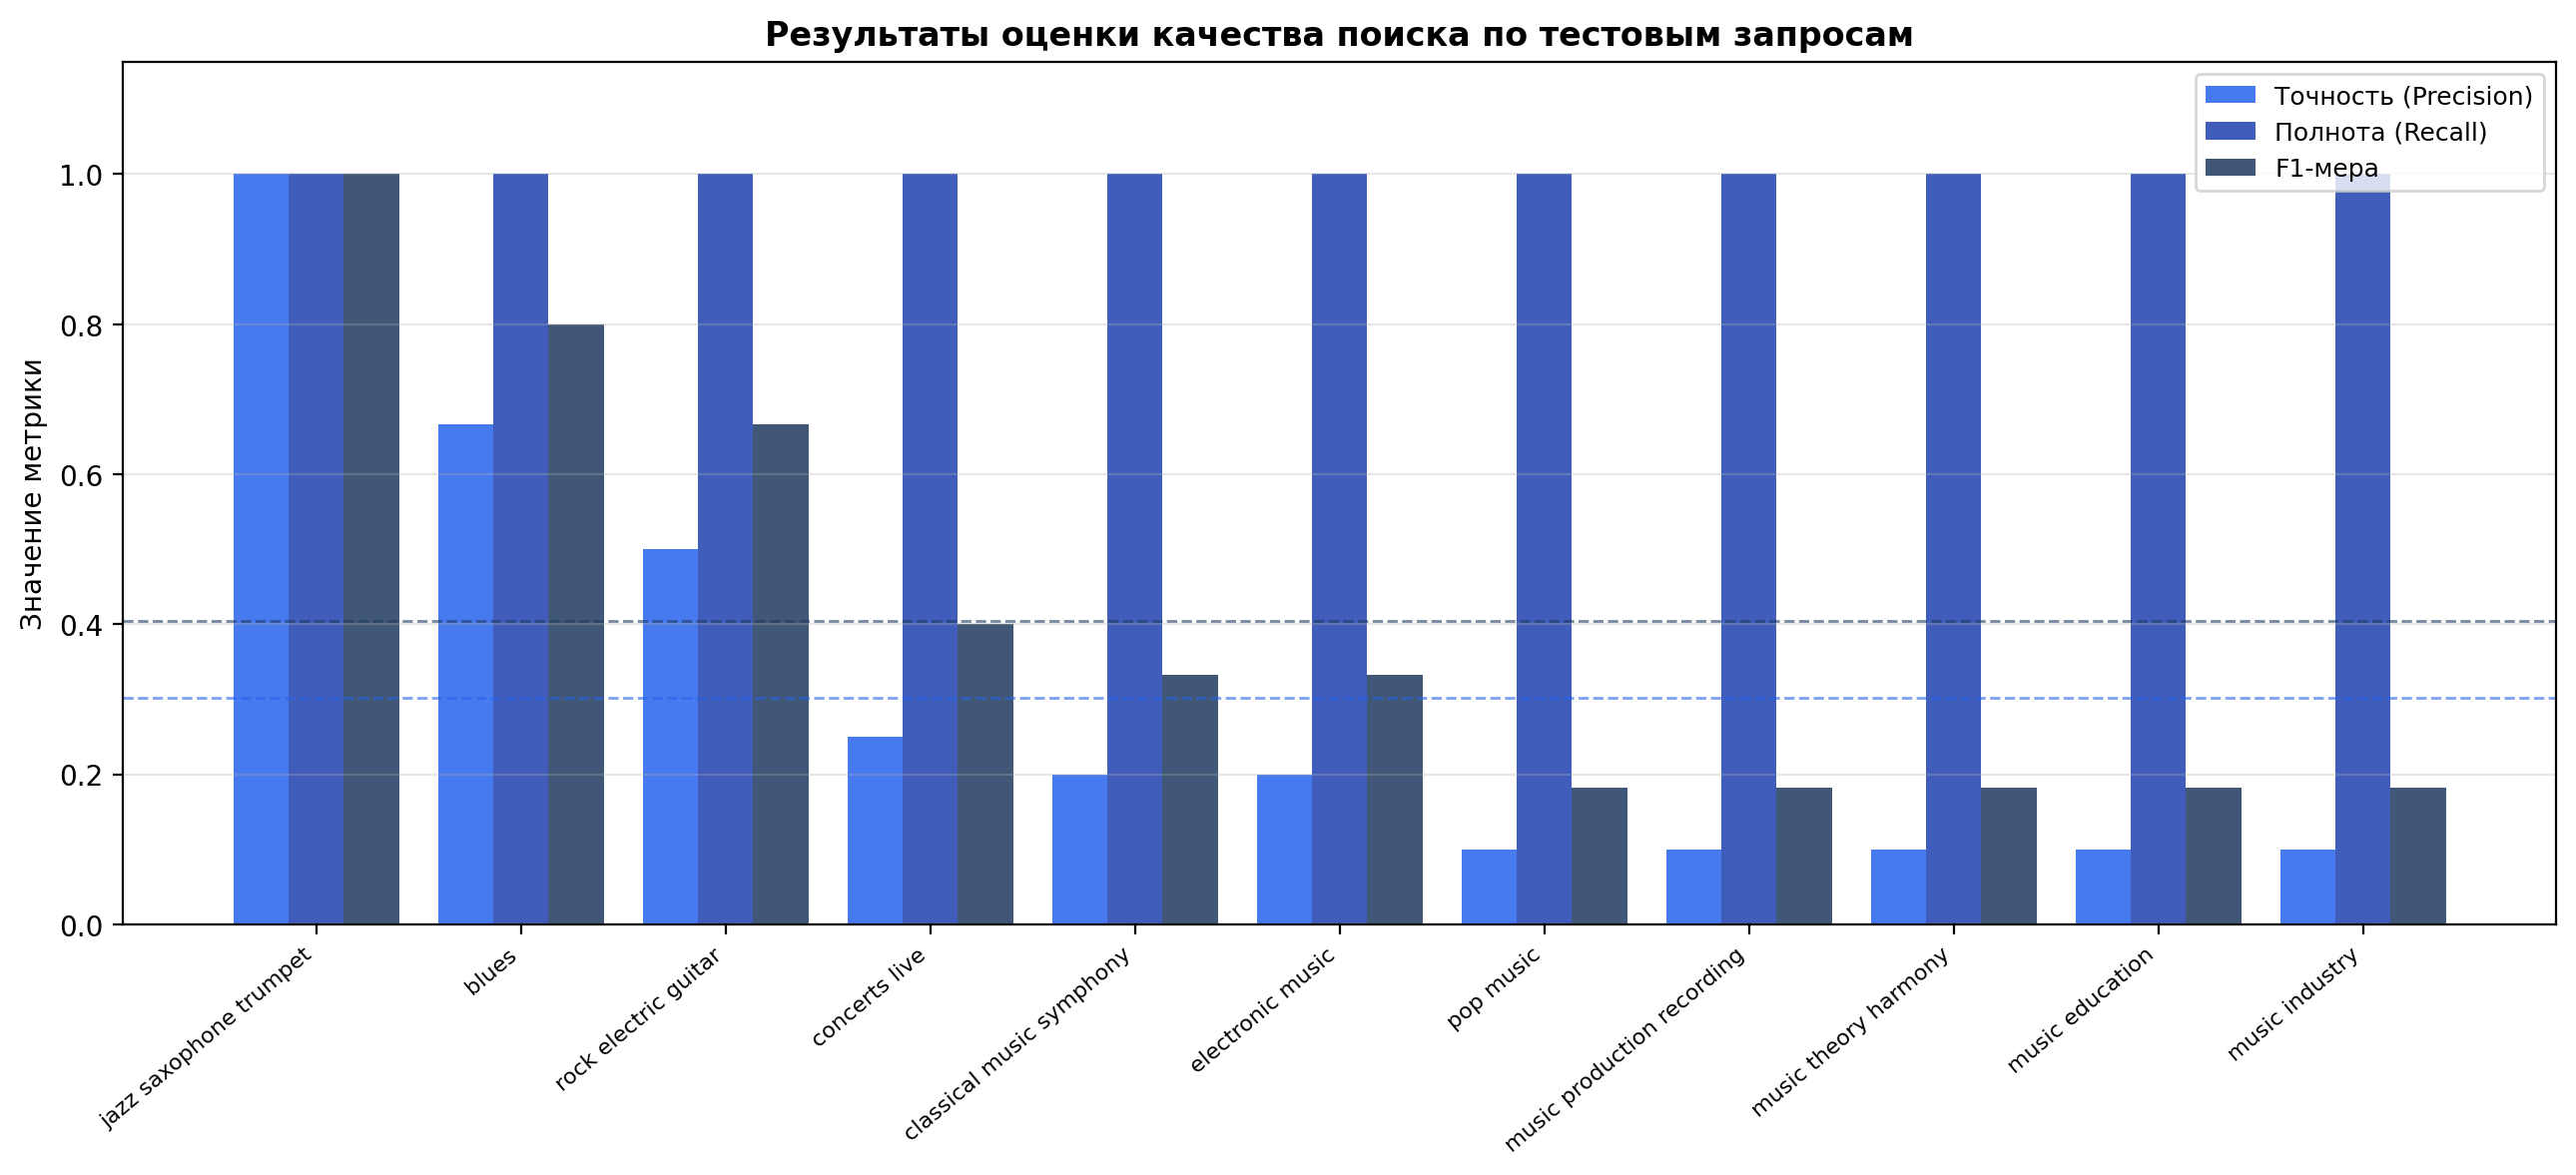
\includegraphics[width=1.0\textwidth]{png/metrics_ru.png}
	\caption{Результаты оценки качества поиска по тестовым запросам.}
	\label{fig:metrics}
\end{figure}

\subsection{Анализ результатов и предложения по улучшению}

Анализ полученных данных показывает следующее:

\begin{itemize}
	\item точность поиска высокая для специфичных запросов с редкими терминами (P = 1,0 для \texttt{jazz saxophone trumpet}) и низкая для общих запросов (P = 0,1), что характерно для векторной модели с TF-IDF на малом тематически однородном корпусе;
	\item полнота во всех случаях равна 1,0 из-за малого размера коллекции; на более крупном корпусе полнота станет информативной метрикой;
	\item фиксированная размерность вектора (5000) при росте словаря потребует согласованного изменения схемы БД и кода приложения.
\end{itemize}

Предложения по улучшению работы системы информационного поиска:

\begin{enumerate}
	\item \textbf{расширение корпуса} "--- увеличение числа и тематического разнообразия документов сделает оценку метрик более репрезентативной и позволит корректно измерять полноту;
	\item \textbf{переход к BM25} "--- вероятностная модель ранжирования Okapi BM25 обычно даёт более высокую точность, чем TF-IDF, особенно для длинных запросов;
	\item \textbf{гибридный поиск} "--- комбинирование векторного поиска (pgvector) с лексическим (BM25/инвертированный индекс) и слиянием результатов, что повышает полноту по точным совпадениям терминов;
	\item \textbf{расширенная предобработка} "--- лемматизация вместо стемминга, обработка чисел и аббревиатур, учёт биграмм/фраз;
	\item \textbf{автоматизация оценки} "--- формирование эталонных релевантностей по документам корпуса и регулярные прогоны метрик (P@k, nDCG, MAP) в CI;
	\item \textbf{отказ от фиксированной размерности} "--- переход на разреженные векторы или пересоздание индекса при росте словаря без ручного вмешательства;
	\item \textbf{уточнение выдач} "--- кластеризация результатов, расширение запросов синонимами, релевантностный фидбек по кликам пользователей;
	\item \textbf{производственный запуск} "--- замена встроенного сервера Flask на gunicorn и включение кэширования для частых запросов.
\end{enumerate}

\subsection{Вывод по разделу}

В рамках раздела реализована информационно-поисковая система с векторной моделью
индексирования на основе TF-IDF и поиском по косинусной близости в PostgreSQL
(pgvector). Система поддерживает загрузку документов в нескольких форматах, поиск с
подсветкой релевантных терминов, просмотр и удаление документов, а также автоматическую
оценку качества по метрикам точности, полноты и F-меры с графическим представлением.
Архитектура разделена на модули по ответственности, развёртывание выполняется в Docker
Compose и доступно в локальной вычислительной сети. Тестирование подтвердило
работоспособность всех сценариев; средняя F1-мера на тестовой коллекции составила 0,404
при полноте 1,0, что позволяет сделать вывод о корректной работе системы и определить
направления её дальнейшего улучшения.
